\documentclass[conference]{IEEEtran}
\IEEEoverridecommandlockouts
% The preceding line is only needed to identify funding in the first footnote. If that is unneeded, please comment it out.
\usepackage{cite}
\usepackage{amsmath,amssymb,amsfonts}
\usepackage{algorithmic}
\usepackage{graphicx}
\usepackage{textcomp}
\usepackage{xcolor}
\def\BibTeX{{\rm B\kern-.05em{\sc i\kern-.025em b}\kern-.08em
    T\kern-.1667em\lower.7ex\hbox{E}\kern-.125emX}}

\ifCLASSINFOpdf
\else
    \usepackage[dvips]{graphicx}
\fi
\usepackage{url}
\usepackage{listings}
% \usepackage[margin=1in]{geometry}
\usepackage{amsmath,amsthm,amssymb}
\usepackage{amsmath,amsthm,amssymb}
\usepackage[spanish]{babel} %Castellanización
\usepackage[T1]{fontenc} %escribe lo del teclado
\usepackage[utf8]{inputenc} %Reconoce algunos símbolos
\usepackage{lmodern} %optimiza algunas fuentes
\usepackage{blkarray}
\graphicspath{ {images/} }
\usepackage{hyperref} % Uso de links

\newcommand{\N}{\mathbb{N}}
\newcommand{\Z}{\mathbb{Z}}
\usepackage{float}
\newenvironment{theorem}[2][Theorem]{\begin{trivlist}
\item[\hskip \labelsep {\bfseries #1}\hskip \labelsep {\bfseries #2.}]}{\end{trivlist}}
\newenvironment{lemma}[2][Lemma]{\begin{trivlist}
\item[\hskip \labelsep {\bfseries #1}\hskip \labelsep {\bfseries #2.}]}{\end{trivlist}}
\newenvironment{exercise}[2][Exercise]{\begin{trivlist}
\item[\hskip \labelsep {\bfseries #1}\hskip \labelsep {\bfseries #2.}]}{\end{trivlist}}
\newenvironment{problem}[2][Problem]{\begin{trivlist}
\item[\hskip \labelsep {\bfseries #1}\hskip \labelsep {\bfseries #2.}]}{\end{trivlist}}
\newenvironment{question}[2][Question]{\begin{trivlist}
\item[\hskip \labelsep {\bfseries #1}\hskip \labelsep {\bfseries #2.}]}{\end{trivlist}}
\newenvironment{corollary}[2][Corollary]{\begin{trivlist}
\item[\hskip \labelsep {\bfseries #1}\hskip \labelsep {\bfseries #2.}]}{\end{trivlist}}
\newcommand*{\defeq}{\stackrel{\text{def}}{=}}
\newenvironment{solution}{\begin{proof}[Solution]}{\end{proof}}
\hyphenation{op-tical net-works semi-conduc-tor}

\newcommand{\argmax}{\operatornamewithlimits{argmax}}


\usepackage[ruled,vlined]{algorithm2e}


\begin{document}

\title{Tarea 5. Optimización, Gradiente Conjugado Lineal}

\author{\IEEEauthorblockN{Oscar Esaú Peralta Rosales}
\IEEEauthorblockA{\textit{Maestría en Computación} \\
\textit{Centro de Investigación en Matemáticas}}
}

\maketitle

\begin{abstract}
En esta tarea se resuelve un problema de optimización cuadrático para el suavizado de ruido sobre
ciertos datos generado de una función, en particular datos son formados con la función
$f(x,y) = x^2 + y^2 + r$ donde $r$ es un término de ruido proveniente de una distribución
uniforme entre 0 y 1. La solución presentada a este problema se aproxima con el uso del
algoritmo de Gradiente Conjundo Lineal.


\end{abstract}

\begin{IEEEkeywords}
Gradiente Conjugado
\end{IEEEkeywords}

\section{Introduction}

El método de Gradiente Conjugado es un método iterativo para solucionar sistemas de ecuaciones
lineales (se puede extender al caso no lineal) de la forma $Ax = b$ dónde $A$ es una matriz simétrica definida positiva. Equivalentemente
puede ser plateado para resolver el problema minimización cuadrático dado por
$min \Phi(x) = \frac{1}{2} x^T A x - b^Tx$. Una de las características de este método es que genera
un conjunto de vectores ${p_0, p_1, \dots, p_l}$ tal que cada uno de ellos comple la propiedad de
ser conjugados de la matriz $A$, es decir que $p_i^T A p_j=0$ para todo $i \ne j$. Además este
conjunto de vectores son mutuamente ortogonales y linealmente independientes.

Dado que ${p_0, p_1, \dots, p_l}$ forman una base entonces la solución al sistema $x*$ puede ser
escrito como una combinación lineal de dicha base, es decir, $x* = \sum \alpha_i p_i$. Luego

\begin{equation*}
	Ax* = b
\end{equation*}

\begin{equation*}
	\sum \alpha_i A p_i = b
\end{equation*}

multiplicando por $p_k$

\begin{equation*}
	p_k^T \sum \alpha_i A p_i = p_k^T b
\end{equation*}

dado que son ortogonales

\begin{equation*}
	\alpha_k p_k^T A p_k = p_k^T b
\end{equation*}

\begin{equation*}
	\alpha_k = \frac{p_k^T b}{p_k^T A p_k}
\end{equation*}

Esto da a una solución $x*$ al sistema en dónde primero calculamos n direcciones conjugadas y luego
calculamos los ceficientes $\alpha_k$. El algoritmo iterativo de Gradiente Conjugado cálcula estas
direcciones y coeficientes en cada paso. En el Apéndice se muestra el pseudo código de este.\\

El problema de optimización cuadrática a resolver es el siguiente:

\begin{equation}
	arg \min_{x} \sum_{i,j} \Big[
		(x_{i,j} - g_{i,j})^2 + \lambda \sum_{(l,m) \in \Omega_{i,j}} (x_{i,j} - x_{l,m})^2
	\Big]
\end{equation}

dónde $\lambda > 0$ es un parámetro de regularizacion dado. $g$ es la función la cual se desea
suavizar (o filtrar el ruido) con $g(x,y) = x^2 + y^2 + r$ donde $r$ es un término de ruido
proveniente de una distribución uniforme entre 0 y 1; ver Fig \ref{img-1}. Y
$\Omega_{i,j} = \{(i+1, j), (i-1, j), (i, j+1), (i, j-1) \}$ es el conjunto de índices formados por
posiciones vecinas a $(i,j)$.

\begin{figure}[htbp]
    \centerline{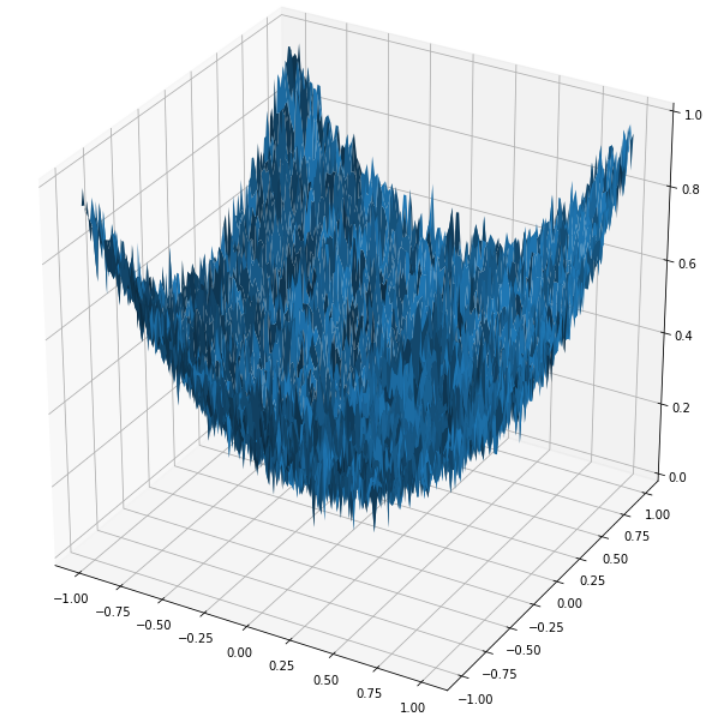
\includegraphics[scale=0.3]{1.png}}
    \caption{Gráfica de $g(x, y)$ con $x,y \in [0,1]$}
    \label{img-1}
\end{figure}

\section{Métodología}

Dado que tenemos que generar valores de nuestra función $g(x, y)$ se fijaron los límites del
problema a los rangos $x_i, y_j \in [0,1]$ así generamos una matriz con valores
$g_{i,j} = g(x_i, y_j)$ de dimensiones $nxm$.

Cómo forma de simplifiación se procedió a representar a la matriz $g$ como un solo
vector (concatenando por renglones) y a reescribir la ecuación (1) de la siguiente forma:

\begin{equation}
	arg \min_{x} f(x) = \sum_{i=0}^{nxm-1} \Big[
		(x_{i} - g_{i})^2 + \lambda \sum_{(k) \in \Omega_{i}} (x_{i} - x_{k})^2
	\Big]
\end{equation}

con $\Omega_i = \{(i+1), (i-1), (i+m), (i-m)\}$. Notemos que en la representación anterior los
vecinos de $x_{i,j}$ estaban localizados en su correspondiente matriz en arriba, abajo, a la
izquierda y a la derecha, en esta nueva los vecinos laterales se conservan en el vector pero los
vecinos de arriba y abajo ahora están a una distancia $\pm m$ en la nueva representación vectorial.
Notemos que las posiciones $k$ en el vector de los vecinos generados deben de estar dentro del rango
$[0, nxm)$ y además los vecinos laterales en alguna posición $k$ de un elemento $i$ también deben
cumplir que $\lfloor k/m \rfloor = \lfloor i/m \rfloor$, es decir, pertenezcan al mismo renglón.

Derivando (2) con respecto a $x_i$ obtenemos que el gradiente es
$\nabla f(x) = [t_1, t_2, \dots, t_{nxm}]^T$ con

\begin{equation}
	t_i = 2(x_i - g_i) + 4\lambda \sum_{k \in \Omega_i} (x_i - x_k)
\end{equation}

y el Hessiano $H$ tal que

\begin{equation*}
	H_{i,i} = 2 + 4 \lambda (\#\Omega_i)
\end{equation*}

\begin{equation*}
	H_{i,i+1} = H_{i,i-1} = H_{i,i+m} = H_{i,i-m} = - 4 \lambda
\end{equation*}

con $\#\Omega_i$ como el numero de vecinos válidos para $x_i$ tal que cumplan las restricciones
sobre el vector mencionadas anteriormente.

Una vez obtenida nuestro nueva representación para el problema se procedió a encontrar una solución
para valores $\lambda=1$, $\lambda=100$ y $\lambda=1000$, los resultados obtenidos se muestran en la
siguiente sección.

Durante la implementación se usó la $Q$ del algoritmo como el Hessiano de la
función y para reducir uso de memoria  procesamiento, dado que $Q$ puede ser una matriz muy grande
en su mayoría con ceros, se implemetó una función que calcula el producto $Qd_k$ en cada iteración.

\section{Resultados}

Se realizaron varias pruebas con valores $\lambda=1$, $\lambda=100$ y $\lambda=1000$ en la tabla
\ref{tab1} se muestra una comparativa de los resultados obtenidos.

\begin{table}[htbp]
    \caption{Tabla comparativa para distintos valores de $\lambda$}
    \begin{center}
        \begin{tabular}{|c|c|c|c|}
            \hline
			\textbf{\textit{$\lambda$}}& \textbf{\textit{Iteraciones}}& \textbf{\textit{$||\nabla g(x*)||$}}& \textbf{\textit{$g(x*)$}} \\

            \hline
            1& 50 & 8.5611e-9 & 27.2598 \\
			100& 101 & 5.9590 & 209.4859 \\
			1000& 103 & 176.67 & 542.67 \\
            \hline
            \multicolumn{4}{l}{}
        \end{tabular}
        \label{tab1}
    \end{center}
\end{table}

Cómo se puede observar con el valor de $\lambda=1$ se alcanzó minimizar el error descrito por
la ecuación (2) mucho mejor que para los otros valores de $\lambda$ y el error más grande se obtuvo
con $\lambda=1000$.

Sin embargo con $\lambda=1$ la poderación al promedio de los errores de los
puntos vecinos tiene muy poca contribución por ello la aproximación a la función es mucho más
precisa y por tanto también el ruido se ve reflejado en esta misma como podemos ver en la Fig
\ref{r1}.

\begin{figure}[htbp]
    \centerline{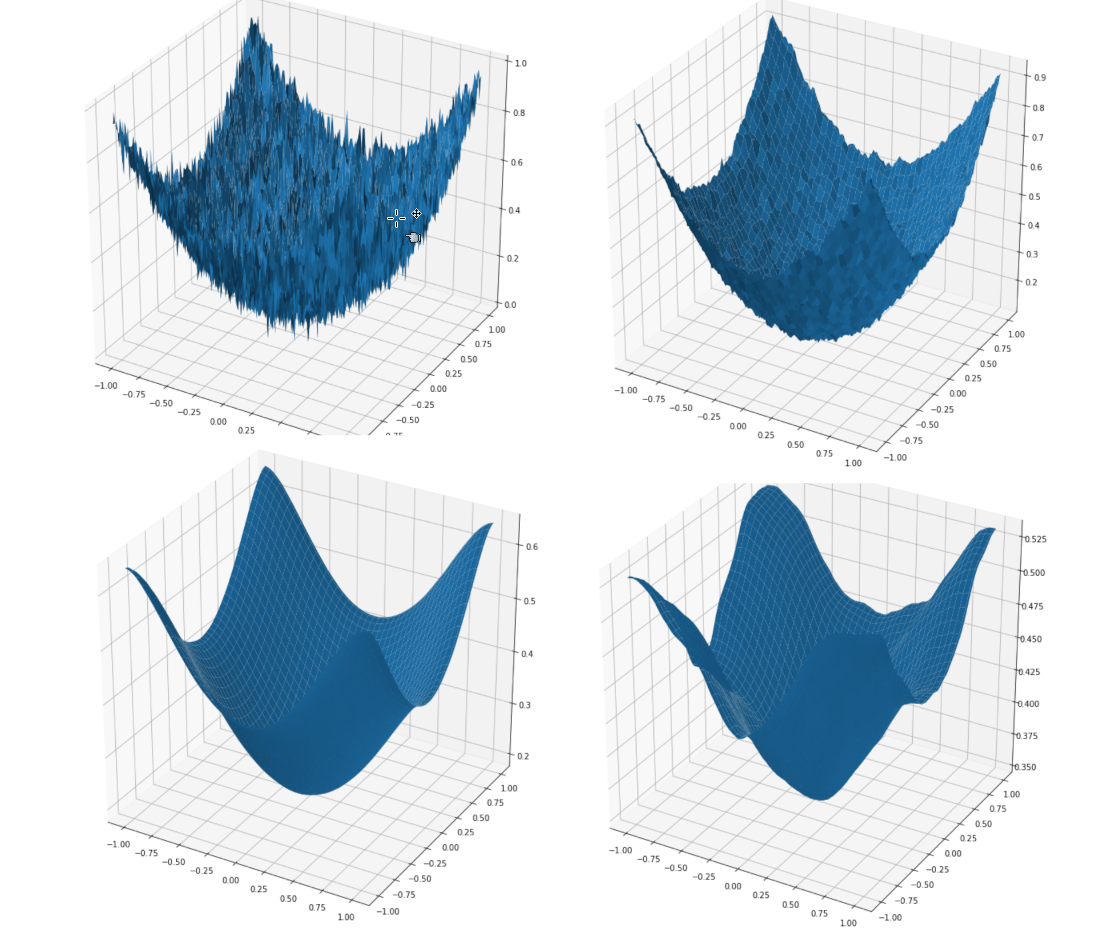
\includegraphics[scale=0.3]{ra.png}}
    \caption{De izquerda a derecha y arriba a abajo; g(x,y), aproximación con $\lambda=1$, aproximación con $\lambda=100$ y aproximación con $\lambda=1000$}
    \label{ra}
\end{figure}

Para $\lambda=100$ se obtuvo un error de aproximación más alto pero como observamos en la figura
\ref{r100} la gráfica es muy similar a la función original sin ruido, esta vez la contribución del
promedio de los errores de los puntos vecinos tiene mayor peso para el calculo del error en un punto
actual, por tanto se espera que el error en esa zona sea mejor promediado suavizando la función
mucho mejor.

Con $\lambda=1000$ el peso del error calculado en un punto tiene menor efecto puesto que dependerá
en mayor medida de la poderación del promedio del error de los pesos de los vecinos provacando que
el suavizado no sea tan \textit{suave} , tal y como se observa en la figura \ref{r1000}.


\section{Conclusiones}

Los resultados obtenidos usando el método de Gradiente Conjugado fueron abstante buenos, en este
caso la funcion a minimizar era una función cuadrática que calculaba el error el error de
aproximación junto con una ponderación del promedio de los errores de los 4 vecinos más cercanos.

Se obtuvo mejores resultados en el savizado usando $\lambda=100$ tal y como se observa en las
figuras \ref{r100} y \ref{ra}, con valore más bajos de lambda la contribución del promediado de los
errores de los vecinas no contribuye demasiado haciedo que la aproximación se ajuste demasiado a la
función original como se vé en la figura \ref{r1} y para valores de $\alpha$ mucho mayores el
suavizado es un poco más abrupto tratándose de parecer más a las regiones de vecinos puesto que
tienen mucho mayor poderación como se observa en la figura \ref{r1000}.

\newpage

\section{Apéndice}

\subsection{Algoritmos}


\begin{algorithm}[h]
    \SetAlgoLined
    \KwResult{$x^*$}
	$x_k$ <- Inicializar \\
	$g_0 = Ax_0 - b$ \\
	$d_0 = -g_0$
    \While{$||g_k|| > tol$}{
		$q_k = Ad_k$\\
		$\alpha_k = \frac{g_k^T g_k}{d_k^T q_k} = - \frac{g_k^T d_k}{d_k^T q_k}$\\
		$x_{k+1} = x_k + \alpha_k d_k$\\
		$g_{k+1} = g_k + \alpha_k q_k = \nabla f(x_{k+1})$\\
		$\beta = \frac{g_{k+1}^T g_{k+1}}{g_k^T g_k} = \frac{g_k^T q_k}{d_k^T q_k}$\\
		$d_{k+1} = - g_{k+1} + \beta_{k+1} d_k$\\
	}
    \caption{Algoritmo Gradiente Conjugado}
\end{algorithm}


\subsection{Gráficos complementarios}

\begin{figure}[htbp]
    \centerline{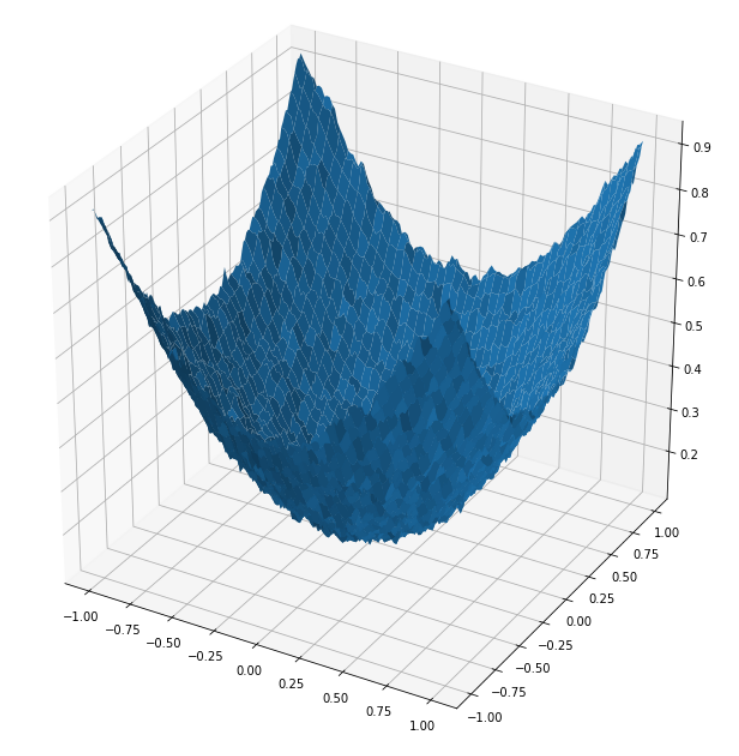
\includegraphics[scale=0.25]{r1.png}}
    \caption{Aproximación a la función con $\lambda=1$}
    \label{r1}
\end{figure}

\begin{figure}[htbp]
    \centerline{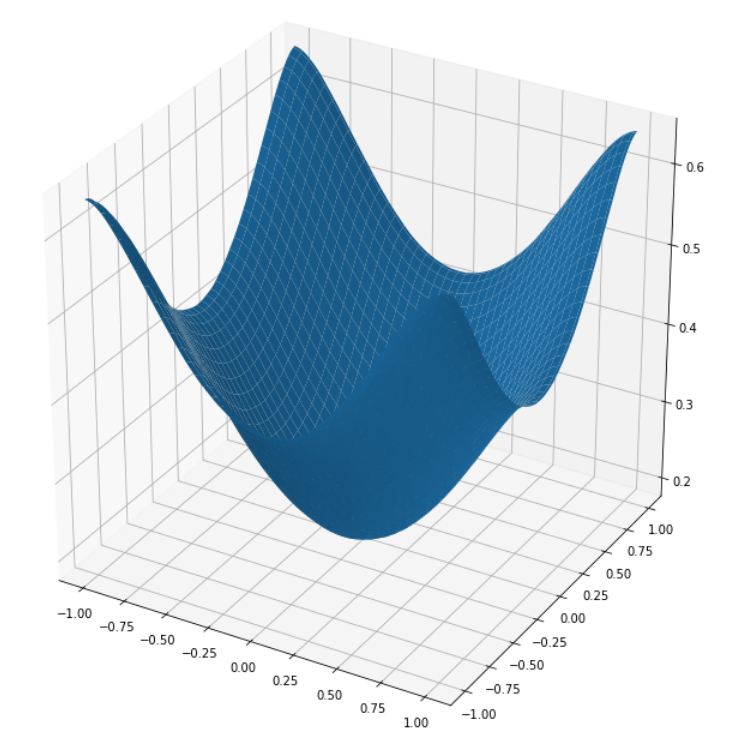
\includegraphics[scale=0.25]{r100.png}}
    \caption{Aproximación a la función con $\lambda=100$}
    \label{r100}
\end{figure}

\begin{figure}[htbp]
    \centerline{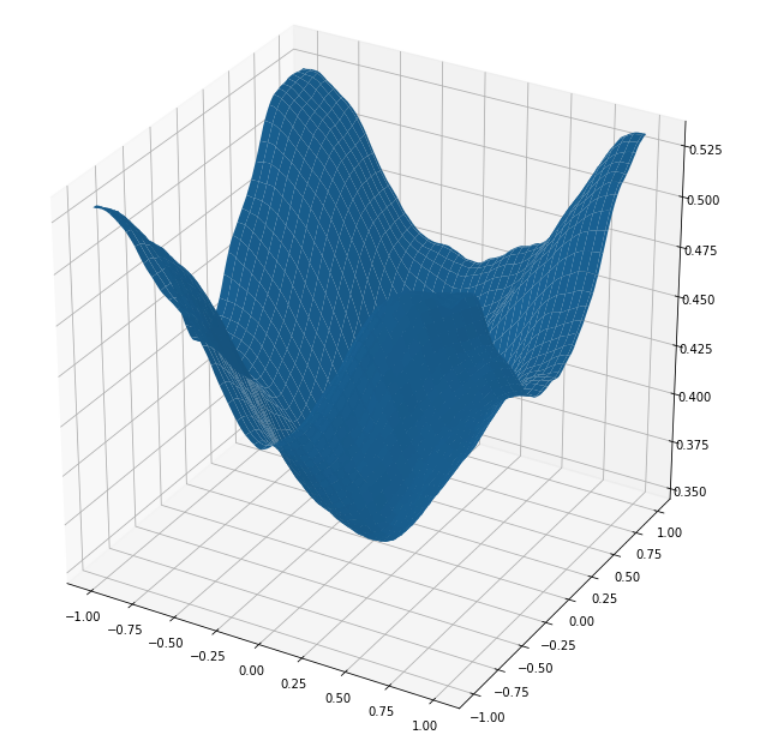
\includegraphics[scale=0.25]{r1000.png}}
    \caption{Aproximación a la función con $\lambda=1000$}
    \label{r1000}
\end{figure}

\begin{figure}[htbp]
    \centerline{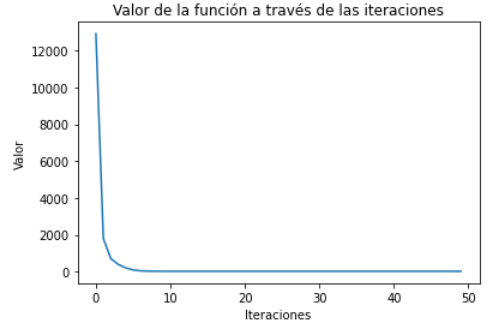
\includegraphics[scale=0.25]{r1f.png}}
    \caption{Grafica de la funcion de error a través de las iteraciones con $\lambda=1$}
    \label{r1f}
\end{figure}

\begin{figure}[htbp]
    \centerline{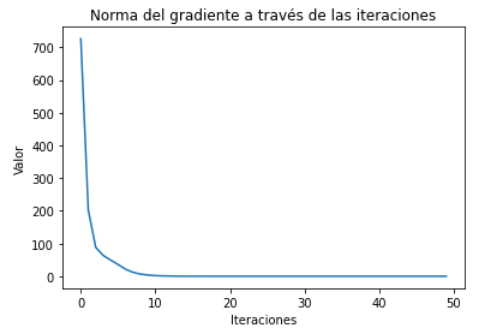
\includegraphics[scale=0.25]{r1g.png}}
    \caption{Grafica de gradiente de la funcion de error a través de las iteraciones con $\lambda=1$}
    \label{r1g}
\end{figure}

\begin{figure}[htbp]
    \centerline{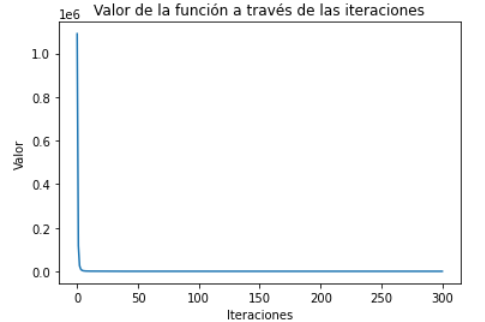
\includegraphics[scale=0.25]{r100f.png}}
    \caption{Grafica de la funcion de error a través de las iteraciones con $\lambda=100$}
    \label{r100f}
\end{figure}

\begin{figure}[htbp]
    \centerline{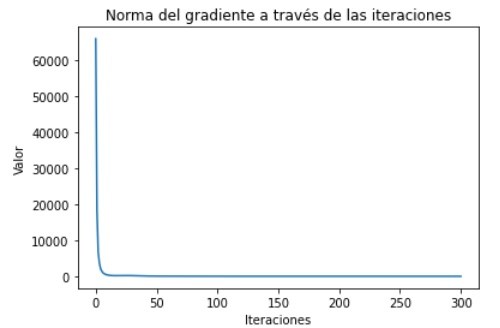
\includegraphics[scale=0.25]{r100g.png}}
    \caption{Grafica de gradiente de la funcion de error a través de las iteraciones con $\lambda=100$}
    \label{r100g}
\end{figure}

\begin{figure}[htbp]
    \centerline{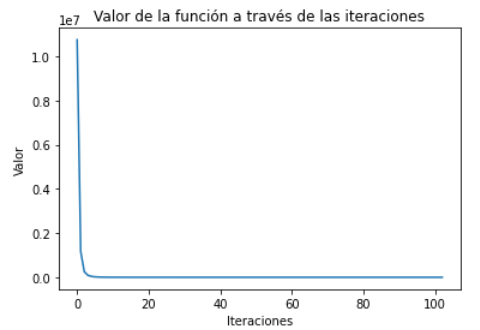
\includegraphics[scale=0.25]{r1000f.png}}
    \caption{Grafica de la funcion de error a través de las iteraciones con $\lambda=1000$}
    \label{r1000f}
\end{figure}

\begin{figure}[htbp]
    \centerline{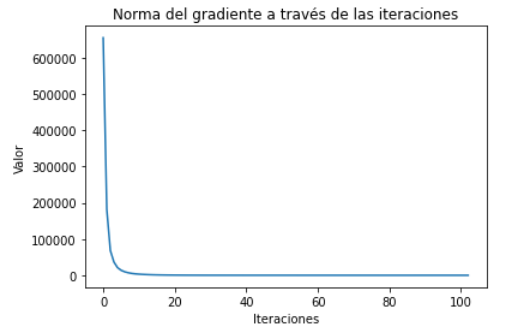
\includegraphics[scale=0.25]{r1000g.png}}
    \caption{Grafica de gradiente de la funcion de error a través de las iteraciones con $\lambda=1000$}
    \label{r1000g}
\end{figure}

\section*{}

\begin{thebibliography}{00}
\bibitem{b1} Jorge Nocedal, Stephen J. Wright, ``Numerical Optimization,'' Second Edition, Springer.
\end{thebibliography}

\end{document}
